% b6c_sizing_formulas.tex
% Formula sheet: sizing of a six-pulse thyristor AC/DC bridge (B6C) with arm fuses, RC snubbers and DC LC output filter
% pwr-control template (AAA_template_latex_settings); numbers of the worked example: b6c_example_calc.py
% Compile: pdflatex b6c_sizing_formulas.tex  (twice, for references)
% Rev. 00 - September 2026 - first issue
% Rev. 01 - 2026-10-03    - RC snubber design criteria (Sec. 5, step S8), bridge-level protection, pwr-control template
\documentclass[10pt,a4paper]{scrartcl}
% ===================== PACKAGES =====================
\usepackage[british]{babel}
\usepackage[tmargin=1in, bmargin=1in, lmargin=0.75in, rmargin=0.75in]{geometry}
\usepackage[dvipsnames,table]{xcolor}  % prima di tikz, listings, ecc.

\usepackage{tikz}
\usepackage{graphicx}
\usepackage{pgfplots}
\pgfplotsset{width=12cm, compat=1.9}
\usepackage{setspace}
\usepackage{chemmacros}
\usepackage{chemfig}
\usepackage{esint}
\usepackage{tabularray}
\usepackage{makeidx}
\usepackage{epstopdf}
\usepackage{amssymb}
\usepackage{mathrsfs}
\usepackage{bm}
\usepackage{amsmath}
\usepackage{enumitem}
\usepackage[english]{varioref}
\usepackage{lipsum}
\usepackage{fancyhdr}
\usepackage{float}
\usepackage{empheq}
\usepackage[framemethod=tikz]{mdframed}
\numberwithin{equation}{section}
\usepackage{eso-pic}
\usepackage{calc}
\usepackage{nccmath}
\usepackage{caption}
\usepackage{subcaption}
\usepackage{gensymb}
\usepackage{amsfonts, amsthm, epsfig, epstopdf, titling, url, array}
\usepackage{tabularx}
\usepackage{makecell}
\usepackage{booktabs}
\usepackage{array}
\usepackage{siunitx}
\sisetup{input-digits=0123456789\pi}
\usepackage[symbol]{footmisc}
\usepackage{multicol}
\usepackage{boondox-cal}
\usepackage{blindtext}
\usepackage{changepage}
\usepackage{nomencl}
\usepackage{hyperref}
\usepackage{xurl}
\usepackage{ragged2e}
\usepackage[version=4]{mhchem}  % ← conflitto di opzioni
\usepackage{longtable}
\usepackage{chemformula}
\usetikzlibrary{arrows.meta,positioning,calc}

% ===================== SI UNITS =====================
\DeclareSIUnit\atm{atm}
\DeclareSIUnit{\var}{var}
\DeclareSIUnit{\pu}{p.u.}


% ===================== MATH OPERATORS =====================
\DeclareMathOperator{\rank}{rank}
\DeclareMathOperator{\atantwo}{atan2}
\DeclareMathOperator{\spn}{span}

% ===================== COMMANDS =====================
\newcommand{\abs}[1]{\left|#1\right|}
\newcommand{\sign}{\text{sign}}
\newcommand{\centered}[1]{\begin{tabular}{@{}l@{}} #1 \end{tabular}}

% ===================== COLORS =====================
\definecolor{mycolor1}{rgb}{0.97, 0.97, 0.97}
\definecolor{mycolor2}{rgb}{0.97, 0.97, 0.97}
\definecolor{tableShade}{gray}{0.9}

% ===================== THEOREM ENVIRONMENTS =====================
\theoremstyle{it}
\newtheorem{defn}{Definition}[section]
\newtheorem{assumption}{Assumption}[section]
\newtheorem{thm}{Theorem}[section]
\newtheorem{lemma}{Lemma}[section]
\newtheorem{corollary}{Corollary}[section]
\theoremstyle{definition}
\newtheorem{example}{Example}[section]

% ===================== CUSTOM ENVIRONMENTS =====================
\newenvironment{myitemize_1}{
	\begin{itemize}[topsep=0pt]
		\setlength{\topsep}{2pt}
		\setlength{\itemsep}{2pt}
		\setlength{\parskip}{2pt}
		\setlength{\parsep}{2pt}
	}{\end{itemize}}

\newmdenv[
innerlinewidth=0.5pt,
roundcorner=4pt,
backgroundcolor=mycolor2,
linecolor=mycolor1,
innerleftmargin=6pt,
innerrightmargin=6pt,
innertopmargin=6pt,
innerbottommargin=6pt
]{mybox}

% ===================== TABLE COLUMN TYPES =====================
\newcolumntype{Y}{>{\hsize=2\hsize}X}
\newcolumntype{Z}{>{\centering\arraybackslash\hsize=0.857\hsize}X}

% ===================== SECTION DEPTH =====================
\setcounter{secnumdepth}{3}
\setcounter{tocdepth}{3}

% ===================== PAGE STYLE =====================
\setlength{\headheight}{20pt}
\setlength{\headsep}{20pt}

\pagestyle{fancy}
\fancypagestyle{firstpage}{\rhead{}}
\fancyhead[L]{\slshape\nouppercase{\leftmark}}
\chead{}
\rhead{\includegraphics[height=0.75cm]{../../AAA_template_latex_settings/pwr-control_logo_doc.png}}
\lfoot{\href{http://www.pwr-control.com}{pwr-control.com}}
\cfoot{-\ \thepage\ -}
\rfoot{\textit{}}
\renewcommand{\headrulewidth}{0.4pt}
\renewcommand{\footrulewidth}{0.4pt}


\geometry{
	a4paper,
	top    = 2.5cm,
	bottom = 3.0cm,
	left   = 2.5cm,
	right  = 2.5cm
}

\hypersetup{
	colorlinks = true,
	urlcolor   = blue,
	linkcolor  = black,
	citecolor  = black
}

\pagenumbering{gobble}
% the document sits three levels below the repository root: logo path of settings.tex corrected here
\rhead{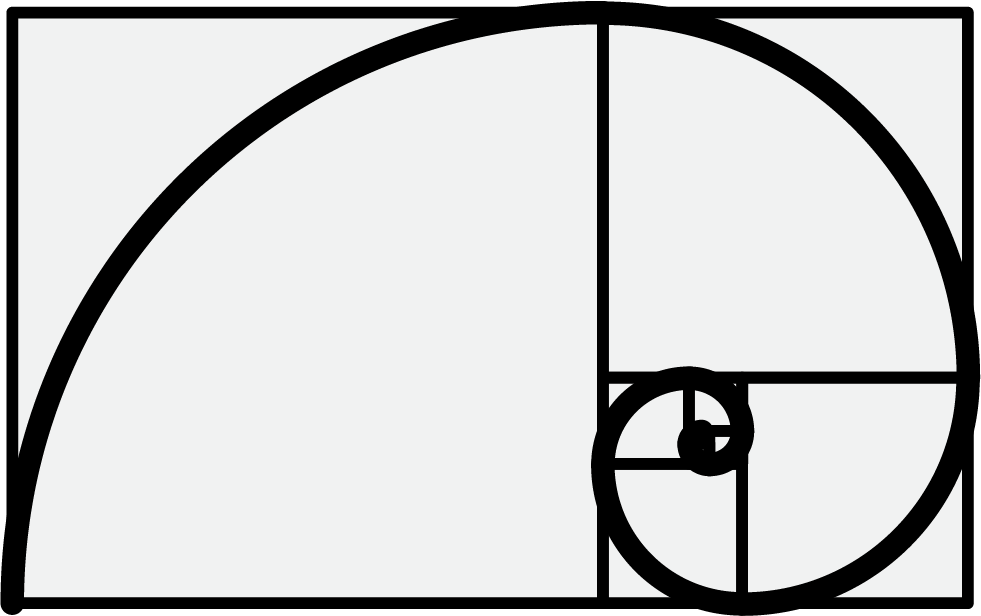
\includegraphics[height=0.75cm]{../../../AAA_template_latex_settings/pwr-control_logo_doc.png}}
\rfoot{\small Rev.~01}
% formula sheet: same text width as the earlier version (17 cm)
\geometry{left=2.0cm, right=2.0cm}
\usetikzlibrary{shapes.geometric,shapes.symbols}

\sisetup{per-mode=symbol,range-phrase={\text{--}},range-units=single}
\setlist{nosep}
\setlength{\parindent}{0pt}
\setlength{\parskip}{3pt}
\allowdisplaybreaks

% --- shorthand ---
\newcommand{\Vdo}{V_{d0}}
\newcommand{\Vd}{V_{d}}
\newcommand{\Id}{I_{d}}
\newcommand{\Vll}{V_{2}}
\newcommand{\Xk}{X_{k}}
\newcommand{\Lk}{L_{k}}
\newcommand{\Rk}{R_{k}}
\newcommand{\uk}{u_{k}}
\newcommand{\ur}{u_{r}}
\newcommand{\Dx}{D_{x}}
\newcommand{\Dr}{D_{r}}
\newcommand{\Dt}{D_{t}}
\newcommand{\ITav}{I_{T\mathrm{(AV)}}}
\newcommand{\ITrms}{I_{T\mathrm{(RMS)}}}
\newcommand{\ITSM}{I_{TSM}}
\newcommand{\VRRM}{V_{RRM}}
\newcommand{\VRSM}{V_{RSM}}
\newcommand{\VDRM}{V_{DRM}}
\newcommand{\iit}{I^{2}t}
\newcommand{\Tj}{T_{j}}
\newcommand{\chk}[1]{\quad\Rightarrow\quad\text{#1}}
\newcommand{\rt}[1]{\text{\small\color{blue!60!black} #1}}

% =============================================================
%  DOCUMENT DATA (title page: AAA_template_latex_settings/titlepage.tex)
% =============================================================
\newcommand{\DocCategory}{Technical Note}
\newcommand{\DocField}{Power Electronics and Control Systems}
\newcommand{\DocTitle}{%
	{\fontsize{20}{24}\selectfont\bfseries Six-Pulse Thyristor Bridge (B6C)} \\[16pt]
	{\fontsize{16}{20}\selectfont\bfseries with Arm Fuses, RC Snubbers and DC LC Filter}
}
\newcommand{\DocSubtitle}{Sizing formula sheet and design path}
\newcommand{\DocAuthor}{Davide Bagnara}
\newcommand{\DocRevision}{01}
\newcommand{\DocDate}{October 2026}
\newcommand{\DocAbstract}{%
Formula sheet and design path for a fully controlled six-pulse thyristor bridge (B6C) fed by a transformer, with one fuse in series with each thyristor, an RC snubber across each thyristor and an LC output filter. The sheet collects, without derivation, the relations needed to size the transformer and the no-load voltage, the firing-angle range, the thyristors (voltage, current, thermal, surge), the RC snubbers, the arm fuses and their $I^2t$ coordination, the DC filter and the grid-side quantities, organised in a fourteen-step iterative sizing path. Revision~01 adds the snubber design criteria: reverse-recovery overvoltage from a normalised snap-off transient, voltage budget, capacitance and optimum damping, $dv/dt$, turn-on discharge, losses and ratings, and the bridge-level protection against the magnetizing energy of the transformer. A worked example (\SI{440}{V}, \SI{1000}{A}) runs the whole path; its numbers are reproduced by the companion Python script.
}
\newcommand{\RevisionHistory}{%
	00 & September 2026 & First issue. & \DocAuthor \\
	01 & October 2026 & RC snubber design criteria (Sec.~5, step S8), bridge-level protection, worked example extended; sizing path renumbered S1--S14; pwr-control template. & \DocAuthor \\
}
\newcommand{\MetaLabelA}{Project Repository}
\newcommand{\MetaValueAUrl}{https://github.com/pwr-control/repositories-documentation.git}
\newcommand{\MetaValueALabel}{repositories-documentation.git}
\newcommand{\MetaLabelB}{Calculation}
\newcommand{\MetaValueB}{Python 3 / NumPy (\texttt{b6c\_example\_calc.py})}

\begin{document}
% =============================================================
%  pwr-control LaTeX template - FRONTESPIZIO
%
%  Da richiamare come prima istruzione dopo \begin{document}:
%      \input{../../AAA_template_latex_settings/titlepage}
%
%  Il documento deve definire prima di \begin{document}:
%      \DocCategory   categoria del documento
%      \DocField      area tecnica
%      \DocTitle      titolo (una o due righe)
%      \DocSubtitle   sottotitolo
%      \DocAuthor     autore/i, separati da virgola
%      \DocRevision   numero di revisione corrente (es. 00)
%      \DocDate       data della revisione corrente
%      \DocAbstract   abstract
%      \RevisionHistory  righe della tabella di revisione, nel formato
%                        Rev. & Date & Description & Authors \\
%      \MetaLabelA \MetaValueAUrl \MetaValueALabel
%      \MetaLabelB \MetaValueB
% =============================================================

\providecommand{\DocCategory}{Technical Research Report}
\providecommand{\DocField}{Power Electronics and Control Systems}
\providecommand{\DocSubtitle}{}
\providecommand{\DocRevision}{00}
\providecommand{\DocAbstract}{}
\providecommand{\RevisionHistory}{%
	\DocRevision & \DocDate & First issue. & \DocAuthor \\
}

\titlepage

% ---- Intestazione centrata ----
\begin{center}
	{\Large\scshape \DocCategory}\\[8pt]
	{\large\scshape \DocField}
\end{center}

\vspace{30pt plus 4pt minus 14pt}
\noindent\rule{\linewidth}{0.8pt}

% ---- Titolo ----
\begin{center}
	\DocTitle
\end{center}

\vspace{4pt}
\noindent\rule{\linewidth}{2.2pt}

% ---- Sottotitolo ----
\begin{center}
	\begin{onehalfspace}
		{\large\itshape \DocSubtitle}
	\end{onehalfspace}
\end{center}

% ---- Authors / Revision / Date ----
\vspace{30pt plus 4pt minus 14pt}

\noindent
\begin{minipage}[t]{0.46\linewidth}
	\raggedright
	\textbf{Authors:}\\[2pt]
	\DocAuthor
\end{minipage}%
\hfill
\begin{minipage}[t]{0.22\linewidth}
	\centering
	\textbf{Revision:}\\[2pt]
	\DocRevision
\end{minipage}%
\hfill
\begin{minipage}[t]{0.30\linewidth}
	\raggedleft
	\textbf{Date:}\\[2pt]
	\DocDate
\end{minipage}

\vspace{10pt}
\noindent\rule{\linewidth}{0.8pt}

% ---- Abstract ----
\vspace{24pt plus 4pt minus 12pt}

\begin{center}
	\begin{minipage}{0.88\linewidth}
		\footnotesize
		\begin{onehalfspace}
			\textbf{Abstract:} \DocAbstract
		\end{onehalfspace}
	\end{minipage}
\end{center}

\vfill

% ---- Revision history ----
\begin{center}
	\begin{minipage}{0.96\linewidth}
		\centering
		{\footnotesize\scshape Revision history}\\[6pt]
		{\footnotesize
			\begin{tabular}{@{}cl>{\raggedright\arraybackslash}p{0.36\linewidth}>{\raggedright\arraybackslash}p{0.28\linewidth}@{}}
				\toprule
				\textbf{Rev.} & \textbf{Date} & \textbf{Description} & \textbf{Authors} \\
				\midrule
				\RevisionHistory
				\bottomrule
			\end{tabular}}
	\end{minipage}
\end{center}

\vspace{18pt plus 4pt minus 10pt}

% ---- Metadati in fondo ----
\noindent
\begin{tabular}{@{} r @{\quad} l @{}}
	\textsc{\MetaLabelA:} & {\href{\MetaValueAUrl}{\MetaValueALabel}} \\[3pt]
	\textsc{\MetaLabelB:} & {\MetaValueB}       \\[3pt]
\end{tabular}

% =============================================================
%  Fine frontespizio
% =============================================================
\newpage
\pagenumbering{arabic}
\setcounter{page}{1}

\tableofcontents
\newpage

\section*{Scope}
Fully controlled six-pulse bridge (B6C, DIN~41761) fed by a transformer (or line reactor), one fuse in series with each thyristor (arm fuse), one RC snubber across each thyristor, and an output LC filter feeding a load with a specified DC voltage ripple. Fundamental frequency $f$, $\omega = 2\pi f$. Formulas are quoted without derivation; ideal commutation is assumed unless the overlap angle $\mu$ appears explicitly. All AC quantities are RMS line-to-line unless noted; the hat denotes a peak value.

\section*{Notation}
\begin{center}\footnotesize
\begin{tabular}{@{}>{$}l<{$}p{5.2cm}>{$}l<{$}p{5.2cm}@{}}
\toprule
\Vd,\Id & DC output voltage, current (mean) & V_1,\Vll & primary, secondary line voltage (RMS) \\
\Vdo & ideal no-load DC voltage at $\alpha=0$ & \Delta V_\pm & grid tolerance ($+$/$-$), p.u. \\
\alpha,\mu,\gamma & firing, overlap, extinction margin angle & \uk,\ur & transformer reactive, resistive p.u. drop \\
\Xk,\Lk,\Rk & commutation reactance / inductance / resistance (per phase, referred to secondary) & S_T,I_2 & transformer rating, secondary current \\
\Dx,\Dr,\Dt & inductive, resistive, semiconductor voltage drops & V_{T0},r_T & thyristor threshold voltage, slope resistance \\
I_{T(AV)},I_{T(RMS)} & thyristor mean, RMS current & \ITSM,\iit_T & surge current (\SI{10}{ms}), thyristor $\iit$ \\
I_{Fn},U_{Fn} & fuse rated current, voltage & \iit_{pa},\iit_{tot} & fuse pre-arcing, total (clearing) $\iit$ \\
I''_{k3},I''_{k2} & three-phase, two-phase initial short-circuit current & \hat U_{arc} & fuse peak arc voltage \\
R_s,C_s & arm snubber resistance, capacitance & Z_0,\omega_{0s},\zeta_s & snubber characteristic impedance, natural frequency, damping ratio \\
Q_{rr},I_{RM},S & recovered charge, peak reverse-recovery current, softness factor $t_b/t_a$ & V_{com},\chi & commutation voltage at turn-off, initial-current factor \\
V_{RM},k_{rep} & repetitive peak voltage at turn-off, its budget (p.u.\ of $\VRRM$) & L_\sigma,I_{dis} & snubber loop inductance, turn-on discharge current \\
i_0,W_m & transformer no-load current (p.u.), magnetizing energy & C_Y & star-equivalent capacitance at the bridge AC terminals \\
L,C,R & filter inductance, capacitance, load resistance $\Vd/\Id$ & f_0,\zeta & filter resonance frequency, damping ratio \\
A_n & peak amplitude of $n$-th harmonic of the bridge output voltage & r_{pp} & specified peak-to-peak ripple, p.u. of $\Vd$ \\
\bottomrule
\end{tabular}
\end{center}

%=====================================================================
\section{Sizing path}
The path is iterative: the transformer no-load voltage depends on the drops, which depend on the transformer; the snubber depends on the commutation inductance, on the firing-angle range and on the voltage class, and may in turn move the voltage class; the fuse coordination depends on the thyristor class, which depends on thermal and fault checks; the filter depends on the worst-case firing angle, which is fixed only after the transformer is chosen. Figure~\ref{fig:flow} shows the loop structure; the step list below gives the equation references.

\begin{enumerate}[label=\textbf{S\arabic*},leftmargin=*]
\item Specification: $\Vd$ (min/max to be regulated), $\Id$ (nominal, minimum, overload profile $I_{ol},t_{ol}$), $r_{pp}$, $V_1 \pm \Delta V$, $f$, grid $S_{sc}$, ambient $T_a$, cooling, regenerative operation yes/no.
\item No-load voltage: first guess $d_x = \uk/2$, $d_r \approx 1.05\,\ur$, $\Dt \approx \SIrange{2}{3}{V}$; compute $\Vdo$ from \eqref{eq:Vdoreq}, $\Vll$ from \eqref{eq:V2}.
\item Transformer: $I_2$, $S_T$ \eqref{eq:ST}; $\Xk,\Rk,\Lk$ \eqref{eq:Xk}; recompute $\Dx,\Dr$ in volts \eqref{eq:Dx}--\eqref{eq:Dr}; back to S2 until $\Vdo$ converges (2--4 iterations).
\item Operating points at $V_1(1-\Delta V_-)$, $V_1$, $V_1(1+\Delta V_+)$: $\alpha$ \eqref{eq:alpha}, $\mu$ \eqref{eq:mu}, $\cos\varphi_1$, $Q$ \eqref{eq:pf}. Check $\alpha \ge \alpha_{min}$ at the worst point; if $\alpha_{max}$ or $Q$ are unacceptable, change $\Vll$, add taps, or change $\uk$ and return to S2.
\item Thyristor voltage class \eqref{eq:VRRM}; first transient clamp level (snubber, MOV), confirmed in S8.
\item Thyristor current and losses \eqref{eq:IT}--\eqref{eq:PT}; junction temperature at nominal and overload \eqref{eq:Tj}--\eqref{eq:Tjol}; heat-sink requirement \eqref{eq:Rth}. Fail $\Rightarrow$ larger device, parallel devices, better cooling.
\item Thyristor fault and dynamic data from the datasheet: $\ITSM$, $\iit_T$ \eqref{eq:i2tT}, $(di/dt)_{crit}$, $(dv/dt)_{crit}$, $Q_{rr}$ and $I_{RM}$ versus $di/dt$ at $T_{j,max}$, $t_q$; check \eqref{eq:didt} with the snubber discharge of S8.
\item RC snubber (Sec.~\ref{sec:snubber}): design point \eqref{eq:Vcom}--\eqref{eq:EL}; $C_s$ from the voltage budget \eqref{eq:budget}--\eqref{eq:Cs} and Table~\ref{tab:snubF}, $R_s$ \eqref{eq:Rs}; checks $dv/dt$ \eqref{eq:dvdt}, turn-on discharge \eqref{eq:Idis}, $V_{RM}$ at the S4 points; losses and ratings \eqref{eq:PRs}--\eqref{eq:Rrat}; bridge-level protection \eqref{eq:Wm}--\eqref{eq:CY}. Fail $\Rightarrow$ other $C_s$/$R_s$, higher voltage class (S5), device with lower $Q_{rr}$ (S7).
\item Prospective fault currents \eqref{eq:Ik3}--\eqref{eq:ip} for the fault cases of Sec.~\ref{sec:faults}.
\item Fuse pre-selection: $I_{Fn}$ \eqref{eq:IFn}, $U_{Fn}$ \eqref{eq:UFn}, breaking capacity, $\hat U_{arc}$ \eqref{eq:Uarc}.
\item Coordination \eqref{eq:coord}--\eqref{eq:cutoff}: fuse $\iit_{tot}$ at the actual voltage and fault current against $k_s\,\iit_T$; non-melting under the overload profile \eqref{eq:nomelt}. Fail $\Rightarrow$ other fuse, larger thyristor (S7), or larger $\Xk$ (S3).
\item DC filter: $A_6(\alpha_{max})$ \eqref{eq:An}, $LC$ product \eqref{eq:LC}, $L_{min}$ for continuous conduction \eqref{eq:Lmin}, $f_0$ placement \eqref{eq:f0}, damping \eqref{eq:zeta}. Fail $\Rightarrow$ change the $L/C$ split, add damping, reconsider $r_{pp}$ or $\alpha_{max}$ (S4).
\item Filter component ratings \eqref{eq:Lrat}--\eqref{eq:inrush}; precharge / soft-start.
\item Verification: grid currents and harmonics \eqref{eq:I1}--\eqref{eq:THD}, reactive power compensation, selectivity with the upstream protection, snubber (simulation with a reverse-recovery device model, $v_T$ measured at commissioning), EMC.
\end{enumerate}

\begin{figure}[p]
\centering
\resizebox{\textwidth}{!}{%
\begin{tikzpicture}[
  node distance=6mm and 4mm,
  blk/.style={rectangle,rounded corners=2pt,draw,align=left,font=\footnotesize,text width=6.0cm,inner sep=4pt,fill=blue!4},
  dec/.style={signal,signal to=east and west,signal pointer angle=110,draw,align=center,font=\footnotesize,text width=5.2cm,inner ysep=4pt,inner xsep=2pt,fill=orange!12},
  term/.style={rectangle,rounded corners=6pt,draw,align=center,font=\footnotesize\bfseries,text width=6.0cm,inner sep=4pt,fill=gray!15},
  arr/.style={-{Latex[length=2mm]},thick},
  back/.style={-{Latex[length=2mm]},thick,red!70!black,dashed},
  lbl/.style={font=\scriptsize,red!70!black,fill=white,inner sep=1pt,align=center},
  vlbl/.style={font=\scriptsize,red!70!black,fill=white,inner sep=1pt,rotate=90,anchor=center,align=center},
  ylbl/.style={font=\scriptsize,fill=white,inner sep=1pt}
]
% ---------- left column ----------
\node[term] (start) {Specification (S1): $\Vd$, $\Id$, $I_{d,min}$, $I_{ol}/t_{ol}$, $r_{pp}$, $V_1\pm\Delta V$, $f$, $S_{sc}$, $T_a$, cooling};
\node[blk,below=of start] (s2) {\textbf{S2 -- No-load voltage.} $d_x\approx\uk/2$, $d_r\approx 1.05\,\ur$, $\Dt$ \\ $\Vdo = \dfrac{\Vd+\Dx+\Dr+\Dt}{\cos\alpha_{min}(1-\Delta V_-)}$, \quad $\Vll=\dfrac{\pi\Vdo}{3\sqrt2}$};
\node[blk,below=of s2] (s3) {\textbf{S3 -- Transformer.} $I_2=0.816\,\Id$, $S_T=1.047\,\Vdo\Id$, $\Xk=\uk\Vll^2/S_T$, $\Rk$, $\Lk$ \\ $\Dx=(3/\pi)\Xk\Id$, $\Dr=2\Rk\Id$};
\node[dec,below=of s3] (d1) {$\Vdo$ converged?};
\node[blk,below=of d1] (s4) {\textbf{S4 -- Operating points} at $V_{1,min}$, $V_1$, $V_{1,max}$: $\alpha$, $\mu$, $\cos\varphi_1$, $Q_1$; $\alpha_{max}=\alpha(V_{1,max})$};
\node[dec,below=of s4] (d2) {$\alpha\ge\alpha_{min}$? \\ $\alpha_{max}$, $Q_1$ acceptable?};
\node[blk,below=of d2] (s5) {\textbf{S5 -- Thyristor voltage.} $\VRRM\ge k_v\sqrt2\,\Vll(1+\Delta V_+)$; transient clamp level (snubber, MOV)};
\node[blk,below=of s5] (s6) {\textbf{S6 -- Thyristor current \& thermal.} $\ITav=\Id/3$, $\ITrms=\Id/\sqrt3$, $P_T$, $\Tj$ (nominal, overload), $R_{thHA}$};
\node[dec,below=of s6] (d3) {$\Tj\le T_{j,max}-\Delta T_m$?};
% ---------- right column ----------
\node[blk,right=1.9cm of start] (s7) {\textbf{S7 -- Thyristor fault / dynamic data.} $\ITSM$, $\iit_T$, $(di/dt)_{crit}$, $(dv/dt)_{crit}$, $Q_{rr}(di/dt)$, $t_q$; check $di/dt$ at turn-on};
\node[blk,below=of s7] (s8) {\textbf{S8 -- RC snubber.} $V_{com,max}$, $I_{RM}$; $\rho\Rightarrow\chi_{max}\Rightarrow C_s$; $R_s=2\zeta_{opt}Z_0$; $dv/dt$, $I_{dis}$, $P_{Rs}$; AC-side RC / MOV for $W_m$};
\node[dec,below=of s8] (d6) {$V_{RM}\le k_{rep}\VRRM$? \\ $dv/dt$, $I_{dis}$, $P_{Rs}$ acceptable?};
\node[blk,below=of d6] (s9) {\textbf{S9 -- Fault currents.} $Z_k$, $I''_{k3}$, $I''_{k2}$ (shorted device), $\kappa$, $i_p$; DC-side short through $2\Lk+L$};
\node[blk,below=of s9] (s10) {\textbf{S10 -- Fuse pre-selection.} $I_{Fn}\ge k_F\,\ITrms$, $U_{Fn}\ge\Vll(1+\Delta V_+)$, breaking capacity $\ge I''_k$, $\hat U_{arc}$};
\node[dec,below=of s10] (d4) {\textbf{S11:} $\iit_{tot,F}(U_2,I''_{k2})\le k_s\iit_T$? \\ $\hat U_{arc}\le\VRSM$? no melting at $I_{ol}$, $t_{ol}$?};
\node[blk,below=of d4] (s12) {\textbf{S12 -- DC filter.} $A_6(\alpha_{max})$; $LC\ge(A_6/\Delta\hat v+1)/\omega_6^2$; $L\ge A_6/(\omega_6 I_{d,min})$; $f_0$ vs $f$, $2f$, $6f$, $f_c$; $\zeta_{min}$};
\node[dec,below=of s12] (d5) {$f_0$ placement, $\zeta_{min}$ acceptable?};
\node[blk,below=of d5] (s13) {\textbf{S13 -- Filter ratings.} $L$: $\Id$, $\Delta\hat I_L$, saturation at $i_p$; $C$: $V_C\ge k_C\Vdo(1+\Delta V_+)$, $I_{C,rms}$, ESR; precharge / soft-start};
\node[blk,below=of s13] (s14) {\textbf{S14 -- Verification.} $I_1$, $I_h$, THD$_i$, $Q_1$ compensation, upstream selectivity, snubber ($v_T$ measured), EMC};
\node[term,below=of s14] (end) {Design frozen};

\foreach \a/\b in {start/s2,s2/s3,s3/d1,d1/s4,s4/d2,d2/s5,s5/s6,s6/d3,s7/s8,s8/d6,d6/s9,s9/s10,s10/d4,d4/s12,s12/d5,d5/s13,s13/s14,s14/end}
  \draw[arr] (\a) -- (\b);
\foreach \d in {d1,d2,d4,d5,d6}
  \node[ylbl,anchor=north west] at ($(\d.south)+(1mm,0)$) {yes};
% column connector: d3 (yes) -> gap -> s7
\coordinate (gap1) at ($(start.east)!0.5!(s7.west)$);
\coordinate (gap2) at ($(gap1)+(-3.5mm,0)$);
\coordinate (gap3) at ($(gap1)+(-7mm,0)$);
\coordinate (top1) at ($(start.north)+(0,5mm)$);
\coordinate (top2) at ($(start.north)+(0,9mm)$);
\coordinate (top3) at ($(start.north)+(0,13mm)$);
\draw[arr] (d3.south) -- ++(0,-4mm) node[ylbl,pos=0.5,right]{yes} -| (gap1 |- top1) -| (s7.north);
% ---------- back loops, left column ----------
\coordinate (chL) at ($(s2.west)+(-5mm,0)$);
\coordinate (chL2) at ($(s2.west)+(-10mm,0)$);
\draw[back] (d1.west) -- (chL |- d1.west) node[lbl,pos=0.5,above]{no} -- (chL |- s2.west) -- (s2.west);
\draw[back] (d2.west) -- (chL2 |- d2.west) node[lbl,pos=0.5,above]{no} -- (chL2 |- s2.south west) node[vlbl,pos=0.6]{$\Vll$, taps, $\uk$} -- ($(s2.south west)+(0,2mm)$);
\draw[back] (d3.west) -- (chL |- d3.west) node[lbl,pos=0.5,above]{no} -- (chL |- s6.west) node[vlbl,pos=0.5]{device, cooling} -- (s6.west);
% ---------- back loops, right column ----------
\coordinate (chR) at ($(s7.east)+(5mm,0)$);
\coordinate (chR2) at ($(s7.east)+(10mm,0)$);
\coordinate (chR3) at ($(s7.east)+(15mm,0)$);
\coordinate (chR4) at ($(s7.east)+(20mm,0)$);
\draw[back] (d6.east) -- (chR |- d6.east) node[lbl,pos=0.5,above]{no} -- (chR |- s8.east) node[vlbl,pos=0.5]{$C_s$, $R_s$\\class (S5)} -- (s8.east);
\draw[back] (d4.east) -- (chR2 |- d4.east) node[lbl,pos=0.5,above]{no} -- (chR2 |- s7.east) node[vlbl,pos=0.5]{other fuse / larger device} -- (s7.east);
\draw[back] (d4.east) -- (chR3 |- d4.east) -- (chR3 |- top2) node[vlbl,pos=0.5]{larger $\Xk$} -- (gap2 |- top2) -- (gap2 |- s3.east) -- (s3.east);
\draw[back] (d5.east) -- (chR |- d5.east) node[lbl,pos=0.5,above]{no} -- (chR |- s12.east) node[vlbl,pos=0.5]{$L/C$ split,\\damping, $r_{pp}$} -- (s12.east);
\draw[back] (d5.east) -- (chR4 |- d5.east) -- (chR4 |- top3) node[vlbl,pos=0.5]{lower $\alpha_{max}$ (taps)} -- (gap3 |- top3) -- (gap3 |- s4.east) -- (s4.east);
\end{tikzpicture}}
\caption{Sizing path. Solid: forward steps; dashed red: iteration loops. Left column S1--S6, right column S7--S14.}
\label{fig:flow}
\end{figure}

%=====================================================================
\section{Transformer and no-load voltage}
\begin{align}
\Vdo &= \frac{3\sqrt2}{\pi}\,\Vll = 1.350\,\Vll, \qquad \Vll = \frac{\pi}{3\sqrt2}\,\Vdo = 0.7405\,\Vdo \label{eq:V2}\\
\Vd &= \Vdo\cos\alpha - \Dx - \Dr - \Dt \label{eq:Vd}\\
\Dx &= \frac{3}{\pi}\Xk\Id = \frac{3}{\pi}\omega\Lk\Id, \qquad d_x = \frac{\Dx}{\Vdo}\Big|_{\Id=I_{dN}} = \frac{\uk}{2} \label{eq:Dx}\\
\Dr &= 2\Rk\Id, \qquad d_r = \frac{\Dr}{\Vdo}\Big|_{\Id=I_{dN}} = \frac{\pi}{3}\ur \approx 1.047\,\ur \label{eq:Dr}\\
\Dt &= 2\,(V_{T0} + r_T\Id) \qquad \rt{(two devices in series; add fuse and busbar resistive drops if relevant)} \label{eq:Dt}
\end{align}
Required no-load voltage, evaluated at the minimum grid voltage and at the DC current for which the full $\Vd$ must be guaranteed (nominal or overload):
\begin{align}
\Vdo^{(V_{1,min})} &\ge \frac{\Vd + \Dx + \Dr + \Dt}{\cos\alpha_{min}}, \qquad
\Vdo = \frac{\Vdo^{(V_{1,min})}}{1-\Delta V_-}, \qquad
n_{tr} = \frac{V_1}{\Vll} \label{eq:Vdoreq}
\end{align}
Transformer ratings (both windings, Dy or Yy, B6 bridge) and commutation impedance:
\begin{align}
I_2 &= \sqrt{\tfrac{2}{3}}\,\Id = 0.816\,\Id, \qquad
S_T = \sqrt3\,\Vll I_2 = \frac{\pi}{3}\Vdo\Id = 1.047\,P_{d0} \label{eq:ST}\\
\Xk &= \uk\frac{\Vll^2}{S_T} + X_{L} + X_{grid}, \qquad
\Rk = \ur\frac{\Vll^2}{S_T}, \qquad
\Lk = \frac{\Xk}{\omega}, \qquad
X_{grid} = \frac{\Vll^2}{S_{sc}}\;\rt{(referred to secondary)} \label{eq:Xk}
\end{align}
$\Xk$ is the total commutation reactance per phase: transformer leakage, line reactor and grid impedance referred to the bridge terminals. The transformer thermal rating must also cover the overload profile and the harmonic content (K-factor or manufacturer derating).

%=====================================================================
\section{Commutation, control angle, power factor}
\begin{align}
\cos\alpha - \cos(\alpha+\mu) &= \frac{\sqrt2\,\Xk\Id}{\Vll} = \frac{2\omega\Lk\Id}{\sqrt2\,\Vll} \label{eq:mu}\\
\alpha(V_1) &= \arccos\frac{\Vd + \Dx + \Dr + \Dt}{\Vdo(V_1)}, \qquad
\alpha_{max} = \alpha(V_{1,max},\,I_{d,min}) \;\rt{(largest ripple)} \label{eq:alpha}\\
\cos\varphi_1 &\approx \frac{\cos\alpha + \cos(\alpha+\mu)}{2}, \qquad
\lambda = \frac{P}{S} \approx \frac{3}{\pi}\cos\varphi_1 = 0.955\cos\varphi_1, \quad
Q_1 = P\tan\varphi_1,\quad P = \Vd\Id \label{eq:pf}
\end{align}
Limits on $\alpha$:
\begin{align}
\alpha_{min} &\approx \SIrange{5}{10}{\degree} \;\rt{(firing reliability, control margin at $V_{1,min}$)} \\
\alpha + \mu + \gamma &\le \SI{180}{\degree},\qquad \gamma \ge \omega t_q + \Delta\gamma \;\rt{(inverter mode only)} \label{eq:gamma}
\end{align}
With a unipolar filter capacitor on the DC side, inverter operation ($\Vd<0$) is not possible; $\alpha$ is then limited to the rectifier range and $\gamma$ is not a constraint.

Turn-on current slope of the incoming thyristor (natural commutation, snubber discharge \eqref{eq:Idis} added separately):
\begin{equation}
\left(\frac{di}{dt}\right)_{on} = \frac{\sqrt2\,\Vll\sin\alpha}{2\Lk} + \left(\frac{di}{dt}\right)_{snubber} \le \left(\frac{di}{dt}\right)_{crit} \label{eq:didt}
\end{equation}

%=====================================================================
\section{Thyristor selection}
\subsection{Voltage}
\begin{align}
\hat V_{2,max} &= \sqrt2\,\Vll(1+\Delta V_+), \qquad
\VRRM = \VDRM \ge k_v\,\hat V_{2,max}, \qquad k_v = 2.0\ldots2.5 \label{eq:VRRM}\\
V_{clamp} &\le \VRRM \;\rt{(MOV / snubber transient level)}, \qquad
\VRSM \ge \hat U_{arc}(U_2) \;\rt{(fuse arc voltage, Sec.~\ref{sec:fuses})}
\end{align}
$k_v\approx2.0$ is acceptable when transients are clamped and verified; $k_v\approx2.5$ otherwise. Standard classes: 1200, 1400, 1600, 1800, 2200, 2800, 4500, 6500~V. The class also fixes the room left to the snubber: the repetitive peak at turn-off is $F\,\hat V_{2,max}\sin(\alpha+\mu)_{max}$ with $F \approx 1.2\ldots1.5$ (Sec.~\ref{sec:snubber}), so that with $k_v = 2$ and a bridge that can run at $\alpha+\mu \approx \SI{90}{\degree}$ the budget \eqref{eq:budget} cannot be met with a practical snubber.

\subsection{Current and losses}
\begin{align}
\ITav &= \frac{\Id}{3}, \qquad
\ITrms = \frac{\Id}{\sqrt3}, \qquad
\text{form factor} = \sqrt3 \;\rt{(\SI{120}{\degree} rectangular)} \label{eq:IT}\\
P_T &= V_{T0}\ITav + r_T\ITrms^2 = \frac{V_{T0}\Id}{3} + \frac{r_T\Id^2}{3} \;(+P_{sw}+P_G,\ \rt{negligible at \SI{50}{Hz}}) \label{eq:PT}
\end{align}
The datasheet $\ITav$ is defined for a \SI{180}{\degree} half-sine at a given case temperature; do not compare it directly with $\Id/3$, use \eqref{eq:PT} with the thermal chain instead.

\subsection{Thermal}
\begin{align}
\Tj &= T_a + P_T\,(R_{thJC} + R_{thCH} + R_{thHA}) \qquad\text{or}\qquad \Tj = T_{hs} + P_T\,(R_{thJC}+R_{thCH}) \label{eq:Tj}\\
R_{thHA} &\le \frac{T_{j,max} - \Delta T_m - T_a}{P_T} - R_{thJC} - R_{thCH}, \qquad \Delta T_m = \SIrange{15}{25}{K} \label{eq:Rth}\\
\Tj(t_{ol}) &= T_{hs} + P_T R_{thJH} + (P_{ol} - P_T)\,Z_{thJH}(t_{ol}), \qquad P_{ol} = \frac{V_{T0}I_{ol}}{3} + \frac{r_T I_{ol}^2}{3} \label{eq:Tjol}
\end{align}
$T_{hs}$ constant if $t_{ol}\ll\tau_{hs}$; otherwise add $(P_{ol}-P_T)\,Z_{thHA}(t_{ol})$. For cyclic loads check $\Delta\Tj$ against the power-cycling capability. With $N_p$ devices in parallel use $\Id/N_p$ with a current-sharing factor (typ.\ 1.1--1.2).

\subsection{\texorpdfstring{Surge, $\iit$, $t_q$}{Surge, I2t, tq}}
\begin{align}
\iit_T &= \frac{\ITSM^2\,t_p}{2}\Big|_{t_p=\SI{10}{ms}} \;\rt{(half-sine)}, \qquad
\iit_T(t) \approx \iit_T\sqrt{\frac{t}{\SI{10}{ms}}} \quad \rt{($t > \SI{10}{ms}$, $I^2\sqrt t$ rule)} \label{eq:i2tT}\\
t_q &\le \frac{\gamma_{min}}{\omega} \;\rt{(inverter mode)}
\end{align}
The dynamic data that size the snubber, $(dv/dt)_{crit}$, $(di/dt)_{crit}$, $Q_{rr}$ and $I_{RM}$ versus $di/dt$ at $T_{j,max}$, are used in Sec.~\ref{sec:snubber}.

%=====================================================================
\section{RC snubbers}\label{sec:snubber}
\subsection{Function and connection}
One series $R_s$--$C_s$ branch across each thyristor (arm snubber), mounted at the device terminals, inside the arm fuse. It must
\begin{enumerate}[label=(\roman*),leftmargin=*]
\item limit the repetitive overvoltage produced when the reverse-recovery current of the outgoing thyristor snaps off in the commutation loop $2\Lk$;
\item keep the rate of rise of forward voltage on the blocking thyristors (commutation notches of the other arms, fast grid transients) below $(dv/dt)_{crit}$;
\item do so without overloading the thyristor at turn-on (capacitor discharge) or the resistor (losses).
\end{enumerate}
Non-repetitive overvoltages (switching of the transformer, grid surges) carry far more energy than the arm snubbers can take and are handled by the bridge-level protection of Sec.~\ref{sec:snubbridge}. Inside the fuse, the turn-on discharge flows through the thyristor only, and an arm whose fuse has cleared is isolated; a snubber across fuse and thyristor would leave an $R_s$--$C_s$ path ($\approx\omega C_s\Vll$) across the open arm. The arm snubbers do not limit the fuse arc voltage: \eqref{eq:Uarc} remains the check. The inductance $L_\sigma$ of the loop thyristor--$C_s$--$R_s$ is not covered by the snubber ($L_\sigma\,di/dt$ appears directly on the device): keep it to tens of nH.

\subsection{Recovery transient}
\begin{align}
V_{com} &= \sqrt2\,\Vll\sin(\alpha+\mu), \qquad
\left(\frac{di}{dt}\right)_{off} = \frac{V_{com}}{2\Lk} \;\rt{(outgoing thyristor at the end of the overlap)} \label{eq:Vcom}\\
I_{RM} &\approx \sqrt{\frac{2\,Q_{rr}\,(di/dt)_{off}}{1+S}}, \qquad
Q_{rr} \approx Q_{rr,ref}\sqrt{\frac{(di/dt)_{off}}{(di/dt)_{ref}}} \;\rt{(datasheet at $T_{j,max}$; scaling only if one point is given)} \label{eq:IRM}\\
E_L &= \tfrac12\,(2\Lk)\,I_{RM}^2 = \frac{Q_{rr}V_{com}}{1+S} \;\rt{(energy released at snap-off, per commutation)} \label{eq:EL}
\end{align}
$V_{com}$, $(di/dt)_{off}$ and $I_{RM}$ all grow with $\alpha+\mu$. If the bridge can run at $\alpha\approx\SI{90}{\degree}$ (soft start from $\alpha\approx\SI{90}{\degree}$, current limit, transients), the design point is $\alpha+\mu = \SI{90}{\degree}$: $V_{com,max} = \hat V_{2,max}$, with $\Id$ of that condition (nominal or current limit) and $Q_{rr}$ at $T_{j,max}$; otherwise $(\alpha+\mu)_{max}$ from S4. The other operating points are checked with the chosen $R_s$, $C_s$.

The method follows \cite{mcmurray,mohan,abb5sya2020} and the diode-bridge note \cite{bagnara_snub}, extended to the firing angle. At snap-off the recovery current is diverted into the snubber (ideal snap-off: conservative for soft-recovery devices). Equivalent circuit: $V_{com}$, $2\Lk$, $R_s$, $C_s$ in series, $i(0) = I_{RM}$, $v_C(0) = 0$:
\begin{align}
Z_0 &= \sqrt{\frac{2\Lk}{C_s}}, \qquad
\omega_{0s} = \frac{1}{\sqrt{2\Lk C_s}}, \qquad
\zeta_s = \frac{R_s}{2Z_0}, \qquad
\chi = \frac{I_{RM}Z_0}{V_{com}} \label{eq:snubpar}\\
v_T(0^+) &= R_sI_{RM}, \qquad
V_{RM} = F(\zeta_s,\chi)\,V_{com}, \qquad
F\big|_{R_s=0} = 1+\sqrt{1+\chi^2} \;\rt{(undamped bound)} \label{eq:VRM}
\end{align}
$F(\zeta_s,\chi)$ is given in Table~\ref{tab:snubF} and Fig.~\ref{fig:snubF} (normalisation of McMurray \cite{mcmurray}). For $\chi\gtrsim0.5$ there is an optimum damping $\zeta_{opt}(\chi)$: below it the $2\Lk$--$C_s$ oscillation dominates the peak, above it the initial step $R_sI_{RM}$. For $\chi<0.5$ (large $V_{com}$, small recovery charge) the peak falls monotonically with $\zeta_s$, and the damping is limited by \eqref{eq:dvdt} and \eqref{eq:Idis} instead. The table reproduces the reference points of \cite{mohan} ($\chi = 1$: $F_{min} = 1.5$ at $R_s\approx1.3\,Z_0$).

\begin{table}[htb]
\centering\footnotesize
\caption{Normalised repetitive peak $F = V_{RM}/V_{com}$ of the snap-off transient \eqref{eq:VRM}, and optimum damping. Computed with \texttt{b6c\_example\_calc.py}.}
\label{tab:snubF}
\begin{tabular}{@{}c*{10}{c}@{}}
\toprule
$\zeta_s$ \textbackslash\ $\chi$ & 0 & 0.25 & 0.5 & 0.75 & 1.0 & 1.25 & 1.5 & 2.0 & 2.5 & 3.0 \\
\midrule
0.3 & 1.45 & 1.47 & 1.52 & 1.60 & 1.72 & 1.86 & 2.01 & 2.35 & 2.72 & 3.09 \\
0.4 & 1.36 & 1.38 & 1.42 & 1.50 & 1.61 & 1.75 & 1.91 & 2.27 & 2.65 & 3.05 \\
0.5 & 1.30 & 1.31 & 1.35 & 1.43 & 1.55 & 1.70 & 1.88 & 2.28 & 2.72 & 3.18 \\
0.6 & 1.25 & 1.26 & 1.30 & 1.38 & 1.51 & 1.69 & 1.91 & 2.43 & 3.00 & 3.60 \\
0.7 & 1.21 & 1.22 & 1.26 & 1.35 & 1.51 & 1.77 & 2.10 & 2.80 & 3.50 & 4.20 \\
0.8 & 1.18 & 1.19 & 1.22 & 1.33 & 1.60 & 2.00 & 2.40 & 3.20 & 4.00 & 4.80 \\
1.0 & 1.14 & 1.14 & 1.18 & 1.50 & 2.00 & 2.50 & 3.00 & 4.00 & 5.00 & 6.00 \\
\midrule
$\zeta_{opt}$ & -- & -- & 1.09 & 0.79 & 0.64 & 0.56 & 0.51 & 0.44 & 0.40 & 0.38 \\
$F_{min}$ & -- & -- & 1.18 & 1.33 & 1.51 & 1.69 & 1.88 & 2.26 & 2.65 & 3.05 \\
\bottomrule
\end{tabular}
\end{table}

\begin{figure}[htb]
\centering
\begin{tikzpicture}
\begin{axis}[width=0.62\textwidth, height=0.40\textwidth,
  xlabel={$\zeta_s = R_s/(2Z_0)$}, ylabel={$F = V_{RM}/V_{com}$},
  xmin=0.2, xmax=1.5, ymin=1, ymax=3, grid=major, grid style={gray!25},
  legend pos=outer north east, legend cell align=left, legend style={font=\scriptsize},
  every axis plot/.append style={thick}]
\addplot[black] coordinates {(0.20,1.572) (0.25,1.506) (0.30,1.451) (0.35,1.404) (0.40,1.364) (0.45,1.329) (0.50,1.298) (0.55,1.272) (0.60,1.249) (0.65,1.228) (0.70,1.210) (0.75,1.194) (0.80,1.180) (0.85,1.167) (0.90,1.155) (0.95,1.145) (1.00,1.135) (1.05,1.127) (1.10,1.119) (1.15,1.112) (1.20,1.105) (1.25,1.099) (1.30,1.094) (1.35,1.089) (1.40,1.084) (1.45,1.080) (1.50,1.076)};
\addlegendentry{$\chi=0$}
\addplot[blue!70!black] coordinates {(0.20,1.649) (0.25,1.577) (0.30,1.516) (0.35,1.465) (0.40,1.421) (0.45,1.383) (0.50,1.350) (0.55,1.321) (0.60,1.296) (0.65,1.274) (0.70,1.255) (0.75,1.238) (0.80,1.224) (0.85,1.211) (0.90,1.200) (0.95,1.191) (1.00,1.184) (1.05,1.179) (1.10,1.177) (1.15,1.181) (1.20,1.201) (1.25,1.250) (1.30,1.300) (1.35,1.350) (1.40,1.400) (1.45,1.450) (1.50,1.500)};
\addlegendentry{$\chi=0.5$}
\addplot[teal!70!black] coordinates {(0.20,1.867) (0.25,1.785) (0.30,1.717) (0.35,1.660) (0.40,1.614) (0.45,1.576) (0.50,1.546) (0.55,1.524) (0.60,1.511) (0.65,1.506) (0.70,1.514) (0.75,1.541) (0.80,1.601) (0.85,1.700) (0.90,1.800) (0.95,1.900) (1.00,2.000) (1.05,2.100) (1.10,2.200) (1.15,2.300) (1.20,2.400) (1.25,2.500) (1.30,2.600) (1.35,2.700) (1.40,2.800) (1.45,2.900) (1.50,3.000)};
\addlegendentry{$\chi=1$}
\addplot[orange!80!black] coordinates {(0.20,2.171) (0.25,2.081) (0.30,2.009) (0.35,1.954) (0.40,1.913) (0.45,1.887) (0.50,1.876) (0.55,1.884) (0.60,1.914) (0.65,1.980) (0.70,2.100) (0.75,2.250) (0.80,2.400) (0.85,2.550) (0.90,2.700) (0.95,2.850) (1.00,3.000) (1.05,3.150) (1.10,3.300) (1.15,3.450) (1.20,3.600) (1.25,3.750) (1.30,3.900) (1.35,4.050)};
\addlegendentry{$\chi=1.5$}
\addplot[red!70!black] coordinates {(0.20,2.520) (0.25,2.423) (0.30,2.350) (0.35,2.299) (0.40,2.269) (0.45,2.261) (0.50,2.280) (0.55,2.332) (0.60,2.431) (0.65,2.600) (0.70,2.800) (0.75,3.000) (0.80,3.200)};
\addlegendentry{$\chi=2$}
\addplot[black,dashed,mark=*,mark size=1.2pt] coordinates {(1.09,1.177) (0.79,1.333) (0.64,1.506) (0.56,1.688) (0.51,1.876) (0.44,2.261) (0.40,2.653)};
\addlegendentry{$\zeta_{opt}(\chi)$}
\end{axis}
\end{tikzpicture}
\caption{Normalised peak voltage at snap-off versus damping, for several initial-current factors $\chi = I_{RM}Z_0/V_{com}$. On the right of each minimum the curve becomes the straight line $2\zeta_s\chi = R_sI_{RM}/V_{com}$ (initial step).}
\label{fig:snubF}
\end{figure}

\subsection{Sizing criteria}
\begin{enumerate}[label=\textbf{C\arabic*},leftmargin=*]
\item \textbf{Voltage budget.} The repetitive peak keeps a margin for the non-repetitive transients clamped at bridge level, for the spread of $Q_{rr}$ and for $L_\sigma$:
\begin{equation}
V_{RM} \le V_{RM,adm} = k_{rep}\VRRM, \quad k_{rep} = 0.5\ldots0.6, \qquad
\rho = \frac{V_{RM,adm}}{V_{com,max}} = \frac{k_{rep}\,k_v}{\sin(\alpha+\mu)_{max}} \label{eq:budget}
\end{equation}
\item \textbf{Capacitance.} Largest admissible $\chi$ from $F_{min}(\chi_{max}) = \rho$ (Table~\ref{tab:snubF}), then
\begin{equation}
C_s \ge 2\Lk\left(\frac{I_{RM}}{\chi_{max}V_{com,max}}\right)^{2}, \qquad
C_s \ge 2\Lk\left(\frac{I_{RM}}{\Delta V_C}\right)^{2},\ \Delta V_C = V_{RM,adm}-V_{com} \;\rt{(energy bound)} \label{eq:Cs}
\end{equation}
The energy bound needs no table and is always on the safe side, by a factor of about 3 to 5 on $C_s$ for $\rho = 1.3\ldots2$; it is the natural choice for diode bridges and small $\alpha$, where $V_{com}$ is small and $\chi$ large. As $V_{com}\to\hat V_{2,max}$ the step $V_{com}$ alone overshoots ($F\ge1.2$ for practical damping), and below $\rho\approx1.3$ no practical snubber meets the budget: raise the class (S5).
\item \textbf{Resistance.} Optimum damping for the chosen $C_s$:
\begin{equation}
R_s = 2\,\zeta_{opt}(\chi)\,Z_0 \;\rt{($\zeta_{opt}\approx0.5\ldots0.8$, i.e.\ $R_s\approx(1\ldots1.6)\,Z_0$, for $\chi = 0.75\ldots1.5$)} \label{eq:Rs}
\end{equation}
A larger $R_s$ (as in tables for small bridges) builds the overvoltage itself through the step $R_sI_{RM}$.
\item \textbf{$dv/dt$.} Forward voltage steps $\Delta V$ applied through $2\Lk$ to a blocking thyristor (initial current zero):
\begin{equation}
\left(\frac{dv}{dt}\right)_{max} = g(\zeta_s)\,\omega_{0s}\Delta V \stackrel{\zeta_s\ge0.5}{=} \frac{R_s\Delta V}{2\Lk} \le \frac{(dv/dt)_{crit}}{k_{dv}}, \quad
k_{dv}\approx2 \;\Rightarrow\; R_s \le \frac{2\Lk\,(dv/dt)_{crit}}{k_{dv}\,\hat V_{2,max}} \label{eq:dvdt}
\end{equation}
$g = 2\zeta_s$ for $\zeta_s\ge0.5$ (maximum at $t=0^+$), $g\approx0.8\ldots0.9$ for $\zeta_s = 0.3\ldots0.4$. $\Delta V = \hat V_{2,max}$ is conservative: the notches caused by the commutations of the other arms are about $\tfrac12\hat V_2\sin\alpha$ per step. The step $R_sI_{RM}$ at snap-off is in the reverse direction and is covered by C1; in rectifier operation the forward voltage returns on the outgoing device at grid rate.
\item \textbf{Turn-on discharge.} At firing $C_s$, charged to $V_T(\alpha)\approx\hat V_2\sin\alpha$, discharges through $R_s$ and the thyristor:
\begin{equation}
I_{dis} = \frac{V_T(\alpha)}{R_s} \le \frac{\hat V_{2,max}}{R_s}, \qquad
\left(\frac{di}{dt}\right)_{dis} \approx \frac{V_T}{L_\sigma}\ \text{for}\ t \lesssim \frac{L_\sigma}{R_s}, \qquad
E_{dis} = \tfrac12 C_sV_T^2 \label{eq:Idis}
\end{equation}
$I_{dis}$ adds to \eqref{eq:didt}; it must stay small compared with the on-state current at which $(di/dt)_{crit}$ is specified and within the manufacturer's recommendation, which gives a lower limit $R_s \ge \hat V_{2,max}/I_{dis,adm}$. An $I_{dis}$ above the latching current helps firing at light load with a large DC inductance. $R_s$ must lie in the window set by \eqref{eq:Idis} and \eqref{eq:dvdt}.
\item \textbf{Losses.} Per cycle each snubber sees the turn-on discharge, the turn-off step, and two half-steps for each of the three commutations of the other arms that move the voltage of the blocking device; a step $\Delta V$ dissipates $\tfrac12C_s\Delta V^2$ in $R_s$ whatever $R_s$:
\begin{equation}
P_{Rs} \approx f\left[\tfrac78\,C_s\hat V_2^2\left(\sin^2\alpha + \sin^2(\alpha+\mu)\right) + E_L\right] \le f\left(1.75\,C_s\hat V_2^2 + E_L\right) \label{eq:PRs}
\end{equation}
The charging current at grid frequency, $\omega C_s\hat V_2$, adds $R_s(\omega C_s\hat V_2)^2/2$ (negligible). Rate $R_s$ for the steady-state worst case ($\alpha_{max}$) and check its thermal transient at $\alpha\approx\SI{90}{\degree}$ (soft start, current limit). A switched simulation of the bridge with ideal thyristors and the data of the worked example (\texttt{b6c\_snubber\_sim.py}) gives $P_{Rs}$ within \SI{6}{\percent} of \eqref{eq:PRs} without $E_L$ for $\alpha = 10\ldots\SI{80}{\degree}$, a forward $dv/dt$ below \SI{40}{\percent} of the bound \eqref{eq:dvdt}, and at $\alpha = \SI{80}{\degree}$ a reverse peak of $1.24\,\hat V_2$ without recovery, against $1.22\,\hat V_2$ from Table~\ref{tab:snubF} ($\chi = 0$).
\item \textbf{Ratings.}
\begin{align}
C_s:&\quad V_{C} \ge V_{RM}\ \rt{(repetitive peak; AC component $\approx\hat V_{2,max}$)}, \qquad
\hat\imath_C = \max(I_{RM},\,I_{dis}) \notag\\
&\quad I_{Cs,rms} = I_{Rs,rms} = \sqrt{P_{Rs}/R_s} \label{eq:Csrat}\\
R_s:&\quad P_{Rs}\ \text{at}\ \alpha_{max}, \qquad
E_{pulse} = \max\!\left(\tfrac12C_s\hat V_{2,max}^2,\ E_L + \tfrac12C_sV_{com}^2\right), \qquad \text{non-inductive} \label{eq:Rrat}
\end{align}
Polypropylene film, self-healing, snubber-rated (pulse $dv/dt \ge \hat\imath_C/C_s$), low ESL. With $N_p$ devices in parallel and one snubber per device, size each one with $2\Lk\to N_p\,2\Lk$ and $(di/dt)_{off}\to(di/dt)_{off}/N_p$ (equal sharing).
\end{enumerate}
If C1 cannot be met with acceptable $C_s$ and losses: higher voltage class (S5), device with lower $Q_{rr}$ or softer recovery (S7). The values belong to the pair snubber--commutation inductance: a change of transformer, line reactor or grid short-circuit power changes $\Lk$ and requires a new check.

\subsection{Bridge-level protection}\label{sec:snubbridge}
Switching off the transformer at no load (primary breaker) releases the magnetizing energy into the capacitance on the secondary side. Upper bound (all the energy into the capacitors, worst distribution among the phases):
\begin{align}
W_m &\approx \frac{i_0\,S_T}{2\omega} \;\rt{(three-phase, linear magnetizing inductance)}, \qquad
\hat V_{max}^2 = \hat V_{2,max}^2 + \frac{4W_m}{C_Y} \label{eq:Wm}\\
C_Y &\ge \frac{2\,i_0\,S_T}{\omega\,(\hat V_{max}^2 - \hat V_{2,max}^2)} \;\rt{(star-equivalent capacitance per phase at the bridge AC terminals, $\hat V$ line-to-line)} \label{eq:CY}
\end{align}
The six arm snubbers give $C_Y\approx2C_s$ (with $p$ and $n$ at the neutral potential), usually far too little. Either an AC-side RC network (star or delta, with a series damping resistor) sized with \eqref{eq:CY}, or MOVs with energy rating $\ge W_m$ (with margin for the number of operations) and clamping voltage below $\VRSM$. $\hat V_{max}\approx(0.7\ldots0.8)\,\VRRM$ is a reasonable target for an event that recurs at every switch-off. MOVs or the AC-side RC also clamp grid surges; an earthed screen between the windings limits the transients transferred capacitively at energization.

%=====================================================================
\section{Arm fuses}\label{sec:fuses}
\subsection{Ratings}
\begin{align}
I_{Fn} &\ge k_F\,\ITrms = k_F\frac{\Id}{\sqrt3}, \qquad
k_F = k_T\,k_{cool}\,k_{cyc} \approx 1.2\ldots1.5 \label{eq:IFn}\\
U_{Fn} &\ge \Vll(1+\Delta V_+) \;\rt{(AC rating; the arm sees the line voltage)}, \qquad
I_{cn} \ge I''_{k,max} \;\rt{(breaking capacity)} \label{eq:UFn}\\
\hat U_{arc}(U_2) &\le \VRSM \;\rt{(conservative; better $\le\VRRM$)} \label{eq:Uarc}\\
P_F &\approx P_{Fn}\left(\frac{\ITrms}{I_{Fn}}\right)^{m},\ m\approx1.6\ldots2 \;\rt{(fuse losses, add to cooling; fuse temperature reduces $\iit_{pa}$)} \label{eq:PF}
\end{align}
$k_T$: ambient / adjacent-component temperature; $k_{cool}$: forced-air or liquid cooling of the fuse (manufacturer data); $k_{cyc}$: cyclic-load fatigue derating (operation at 0.6--0.8 of $I_{Fn}$ for strongly cyclic duty). In a symmetric bridge the arc overvoltage divides over the loop inductances, so healthy devices see only part of $\hat U_{arc}$; \eqref{eq:Uarc} is the usual conservative rule unless a fault-loop simulation is available.

\subsection{Fault cases and prospective currents}\label{sec:faults}
\begin{align}
Z_k &= \sqrt{\Rk^2 + \Xk^2}, \qquad
I''_{k3} = \frac{\Vll(1+\Delta V_+)}{\sqrt3\,Z_k} \approx \frac{I_{2N}}{\uk}(1+\Delta V_+) \;\rt{(DC-side short through the bridge)} \label{eq:Ik3}\\
I''_{k2} &= \frac{\Vll(1+\Delta V_+)}{2Z_k} = \frac{\sqrt3}{2}I''_{k3} \;\rt{(shorted device / misfiring: line-to-line via two arms)} \label{eq:Ik2}\\
\kappa &= 1.02 + 0.98\,e^{-3\Rk/\Xk}, \qquad
i_p = \kappa\sqrt2\,I''_k \;\rt{(peak asymmetric current, no fuse limiting)} \label{eq:ip}\\
\left(\frac{di}{dt}\right)_{fault} &\approx \frac{\sqrt2\,\Vll(1+\Delta V_+)}{2\Lk} \;\rt{(device fault)}, \quad
\left(\frac{di}{dt}\right)_{fault,DC} \approx \frac{\sqrt2\,\Vll(1+\Delta V_+)}{2\Lk + L} \;\rt{(DC-side short, first instants)} \label{eq:didtf}
\end{align}
Cases: (a) thyristor failure or misfiring $\to$ two-phase short through the failed arm and the next fired arm, limited by $2Z_k$ only (worst case for the fuse); (b) DC-side short circuit $\to$ three-phase fed, additionally limited by $L$, shared by the conducting arms; (c) capacitor discharge into a load short does not flow through the arm fuses but stresses $L$ and the load wiring; (d) commutation failure in inverter mode (if applicable).

\subsection{\texorpdfstring{$\iit$ coordination}{I2t coordination}}
\begin{align}
\iit_{tot,F}(U_2) &= \iit_{pa} + \iit_{arc}(U_2) = K_U\!\left(\tfrac{U_2}{U_{Fn}}\right)\cdot \iit_{tot,F}(U_{Fn}), \qquad K_U < 1 \;\rt{(manufacturer curve, incl.\ $\cos\varphi_k$)} \label{eq:KU}\\
\iit_{tot,F}(U_2, I''_{k2}) &\le k_s\,\iit_T, \qquad k_s = 0.7\ldots0.8 \;\rt{(tolerances, $\Tj$ above the datasheet condition)} \label{eq:coord}\\
\hat\imath_{c}(I''_{k2}) &\le \ITSM \;\rt{(cut-off current from the current-limiting curve)} \label{eq:cutoff}\\
t_m(I) &\approx \frac{\iit_{pa}}{I^2} \;\rt{($t_m \lesssim \SI{10}{ms}$, adiabatic)} \\
t_m\!\left(\frac{I_{ol}}{\sqrt3}\right) &\ge (3\ldots5)\,t_{ol} \;\rt{(no melting under overload; time--current curve)} \label{eq:nomelt}
\end{align}
For fault durations beyond one half-cycle compare the fuse time--current characteristic with the $I^2\sqrt t$ curve of the thyristor \eqref{eq:i2tT}, not with a constant $\iit_T$. Upstream selectivity: the arm fuse must clear an internal fault before the upstream breaker or transformer fuse operates; the upstream device must clear the faults the arm fuse cannot see (transformer, busbars).

%=====================================================================
\section{Output LC filter}
\subsection{Harmonic content of the bridge output voltage}
Harmonics of order $n = 6k$ of the fundamental, ideal commutation ($\mu = 0$, conservative), peak amplitude:
\begin{align}
A_n(\alpha) &= \frac{2\Vdo}{n^2-1}\sqrt{1 + (n^2-1)\sin^2\alpha}, \qquad
\omega_n = n\omega, \qquad
A_6(0) = 0.0571\,\Vdo,\quad A_6(\SI{90}{\degree}) = 0.343\,\Vdo \label{eq:An}
\end{align}
Evaluate at $\alpha_{max}$ (maximum grid voltage, minimum load) with $\Vdo(V_{1,max})$; the sixth harmonic dominates. Unfiltered peak-to-peak ripple $\approx 2A_6$. Non-characteristic components at $f$ and $2f$ appear with grid unbalance and firing asymmetry and are \emph{not} attenuated by a filter tuned below $6f$; keep $f_0$ away from them.

\subsection{\texorpdfstring{Attenuation and $LC$ product}{Attenuation and LC product}}
Load approximated by $R = \Vd/\Id$ in parallel with $C$:
\begin{align}
H(j\omega) &= \frac{\hat v_{C}}{\hat v_{d}} = \frac{1}{1 - \omega^2 LC + j\omega L/R}, \qquad
|H(\omega_n)| \approx \frac{1}{\omega_n^2 LC - 1} \;\rt{($\omega_n\gg\omega_0$)} \label{eq:H}\\
\Delta\hat v_{target} &= \frac{r_{pp}\Vd}{2}, \qquad
LC \ge \frac{1}{\omega_6^2}\left(\frac{A_6(\alpha_{max})}{\Delta\hat v_{target}} + 1\right) \label{eq:LC}\\
\Delta v_{pp} &\approx 2\sum_{k} A_{6k}\,|H(\omega_{6k})| \;\rt{(check the 12th; usually $<10\,\%$ of the 6th contribution)}
\end{align}

\subsection{Inductance: continuous conduction and ripple current}
\begin{align}
\Delta\hat I_{L} &= \frac{A_6}{\left|\omega_6 L - 1/(\omega_6 C)\right|} \approx \frac{A_6}{\omega_6 L}, \qquad
L \ge L_{min} = \frac{A_6(\alpha)}{\omega_6\,I_{d,min}} \;\rt{(continuous conduction at $I_{d,min}$)} \label{eq:Lmin}\\
L_{min}\big|_{\alpha=0,\ \text{resistive load}} &= \frac{R_{max}}{105\,\omega} \;\rt{(classic critical inductance)}, \qquad
L \approx (1.2\ldots1.5)\,L_{min} \;\rt{(tolerance, saturation)} \label{eq:ILrip}
\end{align}

\subsection{Resonance placement and damping}
\begin{align}
f_0 &= \frac{1}{2\pi\sqrt{LC}}, \qquad
f_0 \le \frac{6f}{3} \;\rt{(attenuation $\ge 8$ at $6f$)} \label{eq:f0}\\
f_0 &\notin (0.8\ldots1.25)\times\{f,\,2f\} \;\rt{(non-characteristic components)}, \qquad
f_0 \ge (3\ldots5)\,f_{c} \;\rt{(current-loop bandwidth)} \\
\zeta &= \frac{1}{2R}\sqrt{\frac{L}{C}} \;\rt{(load damping, worst at light load $R_{max}$)}, \qquad
\zeta_{min} \ge 0.3\ldots0.5, \qquad
|H|_{max} \approx \frac{1}{2\zeta\sqrt{1-\zeta^2}} \label{eq:zeta}\\
R_{d,opt} &= \sqrt{\frac{L}{C}}\sqrt{\frac{(2+n)(4+3n)}{2n^2(4+n)}}, \qquad
|H|_{max} = \sqrt{\frac{2(2+n)}{n}}, \qquad n = \frac{C_d}{C} \;\rt{($R_d$--$C_d$ branch parallel to $C$)} \label{eq:Rd}\\
\zeta_{p} &= \frac{1}{2R_{p}}\sqrt{\frac{L}{C}} \;\rt{($R_p$ parallel to $L$; zero at $R_p/L$, attenuation $\to 1/(\omega R_p C)$ above it)} \\
|H(j\omega)|,\ &|H(j2\omega)| \;\rt{evaluated with $\zeta_{min}$ ($f$, $2f$ components from unbalance and firing asymmetry)}
\end{align}
If $\zeta_{min}$ is not met by the load alone, add a damping network ($R_d$--$C_d$ branch with $n = 3\ldots5$ is the usual choice; $R_p$--$L_p$ across $L$ if the DC-side capacitance must stay small, see \cite{erickson}) or provide active damping in the current controller. The controller bandwidth of a line-commutated bridge is limited by the firing delay ($T_d\approx 1/(12f)\ldots1/(6f)$), so $f_c$ is typically \SIrange{10}{30}{Hz} at \SI{50}{Hz}; the window $f_c \ll f_0 \ll 6f$ is narrow and must be checked explicitly.

\subsection{Component ratings, precharge}
\begin{align}
\text{Inductor:}\quad & I_{L,dc} = \Id, \qquad I_{L,rms}^2 = \Id^2 + \tfrac12\Delta\hat I_L^2, \qquad
I_{sat} > \max(i_p,\ I_{ol}), \qquad W_L = \tfrac12 L\Id^2 \label{eq:Lrat}\\
\text{Capacitor:}\quad & V_{C} \ge k_C\,\Vdo(1+\Delta V_+),\ k_C=1.1\ldots1.2 \;\rt{($\alpha\to0$ control fault)} \label{eq:Crat}\\
& I_{C,rms} \approx \frac{\Delta\hat I_L}{\sqrt2} \;\rt{(dominant harmonic)}, \qquad P_C = I_{C,rms}^2\,ESR, \qquad \Delta v_{C,pp} = 2A_6|H(\omega_6)| \\
\text{Load step:}\quad & \Delta\hat v_C \approx \Delta I\sqrt{\frac{L}{C}} \;\rt{(load rejection, undamped; reduced by damping and control)} \label{eq:step}\\
\text{Hard start:}\quad & \hat I_{L} \approx \Vdo\sqrt{\frac{C}{L}} + \Id \;\rt{($\alpha=0$; check $\ITSM$, fuse $\iit$, $I_{sat}$; else soft-start from $\alpha\approx\SI{90}{\degree}$)} \label{eq:inrush}
\end{align}

%=====================================================================
\section{Grid-side quantities}
\begin{align}
I_2 &= 0.816\,\Id, \qquad
I_1 = \frac{\sqrt6}{\pi}\Id = 0.780\,\Id, \qquad
I_h = \frac{I_1}{h},\ h = 6k\pm1 \;\rt{(ideal: $\mu=0$, smooth $\Id$)} \label{eq:I1}\\
THD_i &= \sqrt{\frac{I_2^2}{I_1^2}-1} = 0.311, \qquad
S_1 = \sqrt3\,\Vll I_1, \qquad
Q_1 = S_1\sin\varphi_1 \;\rt{(compensation / AC filter design)} \label{eq:THD}
\end{align}
Overlap reduces the high-order $I_h$; DC ripple current increases the 5th and 7th. Grid-side power $P_{ac} = \Vd\Id + P_{loss}$.

%=====================================================================
\section{Rules of thumb}
\begin{center}\small
\begin{tabular}{@{}lll@{}}
\toprule
Quantity & Typical value & Note \\
\midrule
$\alpha_{min}$ & \SIrange{5}{10}{\degree} & firing reliability, control headroom at $V_{1,min}$ \\
$\gamma_{min}$ (inverter) & \SIrange{15}{20}{\degree} & $\ge\omega t_q$ + margin \\
$d_x$, $d_r$, $\Dt$ & $\uk/2$, $1.05\,\ur$, \SIrange{2}{3}{V} & first-pass drops \\
$S_T$ & $1.05\,P_{d0}$ & B6, both windings \\
$k_v = \VRRM/\hat V_{2,max}$ & 2.0--2.5 & 2.0 only with verified clamping and $\alpha+\mu\ll\SI{90}{\degree}$ \\
$\Tj$ design margin & \SIrange{15}{25}{K} below $T_{j,max}$ & plus power-cycling check \\
Snubber design point & $\alpha+\mu = \SI{90}{\degree}$ & if soft start or current limit reach it \\
$k_{rep} = V_{RM}/\VRRM$ & 0.5--0.6 & repetitive peak at turn-off \\
$\zeta_s$, $R_s$ & 0.5--0.8, $(1\ldots1.6)\,Z_0$ & $\zeta_{opt}(\chi)$, Table~\ref{tab:snubF} \\
$C_s$ & $2\Lk\,(I_{RM}/\chi_{max}V_{com})^2$ & energy bound 3--5$\times$ larger \\
$(dv/dt)_{max}$ & $R_s\hat V_{2,max}/(2\Lk)$ & $\le(dv/dt)_{crit}/2$ \\
$P_{Rs}$ & $\le f\,(1.75\,C_s\hat V_2^2 + E_L)$ & maximum at $\alpha\approx\SI{90}{\degree}$ \\
$L_\sigma$ (snubber loop) & tens of nH & at the device, inside the fuse \\
AC side & RC or MOV for $W_m = i_0S_T/(2\omega)$ & arm snubbers alone insufficient \\
$k_F$ (fuse derating) & 1.2--1.5 & temperature, cooling, cyclic duty \\
$k_s$ ($\iit$ margin) & 0.7--0.8 & fuse $\iit_{tot}$ at actual $U_2$ \\
$\hat U_{arc}$ & $\le\VRSM$ & conservative \\
$f_0$ & $\le 2f$ (i.e. $6f/3$), away from $f$, $2f$ & attenuation $\ge 8$ at $6f$ \\
$\zeta_{min}$ & 0.3--0.5 & at minimum load \\
$L$ & $(1.2\ldots1.5)\,L_{min}$ & continuous conduction at $I_{d,min}$ \\
$V_C$ & $(1.1\ldots1.2)\,\Vdo(1+\Delta V_+)$ & control fault at $\alpha\to0$ \\
$THD_i$ & \SI{31}{\percent} & ideal six-pulse; $I_h\approx I_1/h$ \\
Start & soft-start from $\alpha\approx\SI{90}{\degree}$ & or precharge circuit \\
\bottomrule
\end{tabular}
\end{center}

%=====================================================================
\section{Worked example}
Specification: $\Vd = \SI{440}{V}$, $\Id = \SI{1000}{A}$, $I_{d,min} = \SI{100}{A}$, overload $1.5\times$ for \SI{60}{s}, grid $\SI{400}{V}\pm\SI{10}{\percent}$, \SI{50}{Hz}, transformer $\uk = \SI{6}{\percent}$, $\ur = \SI{1}{\percent}$, $i_0 = \SI{1.5}{\percent}$ (assumed), $\alpha_{min} = \SI{10}{\degree}$, $r_{pp} = \SI{3}{\percent}$, soft start from $\alpha\approx\SI{90}{\degree}$. Representative thyristor data (not a specific part): $V_{T0} = \SI{0.85}{V}$, $r_T = \SI{0.35}{m\ohm}$, $R_{thJC} = \SI{0.030}{K/W}$, $R_{thCH} = \SI{0.010}{K/W}$, $\ITSM = \SI{15}{kA}$ (\SI{10}{ms}) $\Rightarrow$ $\iit_T = \SI{1.13e6}{A^2 s}$; $Q_{rr} = \SI{1.0}{mC}$ at \SI{10}{A/\micro s} and $T_{j,max}$, $S = 0.3$, $(dv/dt)_{crit} = \SI{500}{V/\micro s}$, $(di/dt)_{crit} = \SI{150}{A/\micro s}$. All figures are reproduced by \texttt{b6c\_example\_calc.py}; \texttt{b6c\_snubber\_sim.py} simulates the bridge with its snubbers.

{\small
\begin{longtable}{@{}l>{\raggedright\arraybackslash}p{0.26\textwidth}>{\raggedright\arraybackslash}p{0.62\textwidth}@{}}
\toprule
Step & Equation & Result \\
\midrule
\endfirsthead
\toprule
Step & Equation & Result \\
\midrule
\endhead
\bottomrule
\endlastfoot
S2--S3 & \eqref{eq:Vdoreq}, \eqref{eq:V2}, \eqref{eq:ST}, \eqref{eq:Xk}, iterated & $\Vdo = \SI{523}{V}$ (first guess \SI{447}{V}, 5 iterations to \SI{1}{mV}); $\Vll = \SI{387}{V}$, $n_{tr} = 1.033$; $I_2 = \SI{816}{A}$, $S_T = \SI{548}{kVA}$; $\Xk = \SI{16.4}{m\ohm}$, $\Lk = \SI{52}{\micro H}$, $\Rk = \SI{2.7}{m\ohm}$ \\
Drops & \eqref{eq:Dx}--\eqref{eq:Dt} & $\Dx = \SI{15.7}{V}$ ($d_x = \SI{3.0}{\percent}$), $\Dr = \SI{5.5}{V}$ ($d_r = \SI{1.05}{\percent}$), $\Dt = \SI{2.4}{V}$ \\
S4 & \eqref{eq:alpha}, \eqref{eq:mu}, \eqref{eq:pf} at $V_1 = 360/400/\SI{440}{V}$ & $\alpha = 10.0/27.6/\SI{36.3}{\degree}$; $\mu = 13.3/6.7/\SI{5.0}{\degree}$; $\cos\varphi_1 = 0.951/0.856/0.778$; $Q_1 = 142/265/\SI{355}{kvar}$ (taps or compensation advisable) \\
S5 & \eqref{eq:VRRM} & $\hat V_{2,max} = \SI{602}{V}$; $\VRRM \ge 1205$ ($k_v = 2$) \ldots \SI{1506}{V} ($k_v = 2.5$) $\Rightarrow$ \SI{1600}{V} class ($k_v = 2.66$; \SI{1800}{V} if $\hat U_{arc}$ or the snubber require) \\
S6 & \eqref{eq:IT}, \eqref{eq:PT}, \eqref{eq:Tj}--\eqref{eq:Tjol} & $\ITav = \SI{333}{A}$, $\ITrms = \SI{577}{A}$, $P_T = \SI{400}{W}$; overload $500/\SI{866}{A}$, $P_{ol} = \SI{688}{W}$; $\Tj = \SI{86}{\celsius}$ at $T_{hs} = \SI{70}{\celsius}$, \SI{98}{\celsius} at overload ($T_{hs}$ constant); $R_{thHA} \le \SI{0.135}{K/W}$ per device for $T_a = \SI{40}{\celsius}$, $\Tj \le \SI{110}{\celsius}$ \\
S7 & \eqref{eq:didt} & $(di/dt)_{on} = 0.8\ldots\SI{3.4}{A/\micro s}$ ($\alpha = 10\ldots\SI{36}{\degree}$), plus the snubber discharge of S8 ($I_{dis}\le\SI{73}{A}$) \\
S8 & \eqref{eq:Vcom}--\eqref{eq:EL} & Design point $\alpha+\mu = \SI{90}{\degree}$ (soft start, current limit) at $\Id = \SI{1000}{A}$: $V_{com} = \SI{602}{V}$, $(di/dt)_{off} = \SI{5.8}{A/\micro s}$, $Q_{rr} = \SI{0.76}{mC}$, $I_{RM} = \SI{82}{A}$, $E_L = \SI{0.35}{J}$ \\
 & \eqref{eq:budget}--\eqref{eq:Rs}, Table~\ref{tab:snubF} & $V_{RM,adm} = 0.55\times1600 = \SI{880}{V}$, $\rho = 1.46$ $\Rightarrow$ $\chi_{max} = 0.94$, $C_s \ge \SI{2.2}{\micro F}$ (energy bound \SI{9.1}{\micro F}) $\Rightarrow$ $C_s = \SI{2.7}{\micro F}$; $Z_0 = \SI{6.2}{\ohm}$, $\chi = 0.85$, $\zeta_{opt} = 0.72$ $\Rightarrow$ $R_s = \SI{8.2}{\ohm}$ ($\zeta_s = 0.66$, $f_{0s} = \SI{9.5}{kHz}$); $V_{RM} = \SI{847}{V} = 0.53\,\VRRM$ \\
 & \eqref{eq:dvdt}, \eqref{eq:Idis} & $(dv/dt)_{max} = \SI{47}{V/\micro s}$ ($R_s \le \SI{43}{\ohm}$ with $k_{dv} = 2$); $I_{dis} = \SI{73}{A}$, $E_{dis} = \SI{0.49}{J}$; at the S4 points ($\alpha+\mu = 23/34/\SI{41}{\degree}$): $V_{RM} = 314/465/\SI{582}{V}$ \\
 & \eqref{eq:PRs}--\eqref{eq:Rrat} & $P_{Rs} = 9/25/\SI{43}{W}$ at the S4 points, \SI{103}{W} at $\alpha = \SI{90}{\degree}$ (six snubbers: \SI{0.26}{kW} in steady state); $I_{Cs,rms} = \SI{2.3}{A}$ (\SI{3.6}{A} at \SI{90}{\degree}), $\hat\imath_C = \SI{82}{A}$, $E_{pulse} = \SI{0.84}{J}$ $\Rightarrow$ $C_s$: \SI{2.7}{\micro F} PP film, $\ge\SI{1.2}{kV}$ DC, snubber-rated; $R_s$: \SI{8.2}{\ohm}, \SI{100}{W} class, non-inductive \\
 & Alternative & \SI{1800}{V} class: $V_{RM,adm} = \SI{990}{V}$, $\rho = 1.64$ $\Rightarrow$ $C_s = \SI{1.5}{\micro F}$, $R_s = \SI{10}{\ohm}$, $V_{RM} = \SI{967}{V}$, $P_{Rs} = \SI{28}{W}$ (\SI{65}{W} at \SI{90}{\degree}) \\
 & \eqref{eq:Wm}, \eqref{eq:CY} & $W_m = \SI{13}{J}$; arm snubbers alone ($C_Y = 2C_s = \SI{5.4}{\micro F}$): up to \SI{3.2}{kV} $\Rightarrow$ AC-side RC with $C_Y \ge \SI{49}{\micro F}$ per phase for $\hat V_{max} = 0.75\,\VRRM = \SI{1.2}{kV}$ ($Q_C = \SI{2.3}{kvar}$), or MOVs $\ge\SI{13}{J}$ per operation with margin \\
S9 & \eqref{eq:Ik3}--\eqref{eq:didtf} at $V_{1,max}$ & $Z_k = \SI{16.7}{m\ohm}$, $X/R = 6$; $I''_{k3} = \SI{14.8}{kA}$, $I''_{k2} = \SI{12.8}{kA}$; $\kappa = 1.61$, $i_p = \SI{29}{kA}$; device-fault $di/dt = \SI{5.8}{A/\micro s}$; DC-side short $di/dt \approx \SI{0.55}{A/\micro s}$ with $L = \SI{1}{mH}$ \\
S10 & \eqref{eq:IFn}--\eqref{eq:Uarc} & $I_{Fn} \ge 1.3\times577 = \SI{751}{A} \Rightarrow \SI{800}{A}$; $U_{Fn} \ge \SI{426}{V} \Rightarrow$ 500 or \SI{690}{V} class; $I_{cn} \ge \SI{15}{kA}$ \\
S11 & \eqref{eq:coord}--\eqref{eq:nomelt} & Requirement: $\iit_{tot,F}(\SI{426}{V},\,\SI{12.8}{kA}) \le 0.8\times\num{1.13e6} = \SI{0.90e6}{A^2 s}$, $\hat\imath_c \le \SI{15}{kA}$, $\hat U_{arc} \le \VRSM$, $t_m(\SI{866}{A}) \ge \SIrange{3}{5}{min}$ -- verify on the fuse curves \\
S12 & \eqref{eq:An}, \eqref{eq:LC}, \eqref{eq:Lmin}, \eqref{eq:f0} & $\alpha_{max} = \SI{36.3}{\degree}$, $\Vdo = \SI{575}{V}$: $A_6 = \SI{120}{V}$, $A_{12} = \SI{57}{V}$; $\Delta\hat v_{target} = \SI{6.6}{V}$ $\Rightarrow$ $LC \ge \SI{5.4e-6}{s^2}$ ($f_0 \le \SI{69}{Hz}$); $L_{min} = \SI{0.64}{mH}$ $\Rightarrow$ $L = \SI{1.0}{mH}$, $C = \SI{5.6}{mF}$, $f_0 = \SI{67}{Hz}$ \\
Check & \eqref{eq:H}, \eqref{eq:zeta} & $|H(6f)| = 0.052$: ripple \SI{12.4}{V} pp = \SI{2.8}{\percent}; 12th adds \SI{0.7}{V}; $\zeta = 0.48$ at full load, $0.05$ at \SI{10}{\percent} load $\Rightarrow$ damping network required; $|H(f)| = 1.2$ (2.2 at \SI{10}{\percent}), $|H(2f)| = 0.53$ (0.82): components at $f$, $2f$ pass -- limit unbalance/asymmetry or move $f_0$ (e.g. $\le\SI{35}{Hz}$ with $C \approx \SI{20}{mF}$) \\
S13 & \eqref{eq:Lrat}--\eqref{eq:inrush} & $\Delta\hat I_L = \SI{67}{A}$, $I_{C,rms} \approx \SI{47}{A}$; $V_C \ge 1.1\times575 = \SI{633}{V}$ $\Rightarrow$ 700--\SI{800}{V} class; hard start $\hat I_L \approx 1360 + 1000 = \SI{2360}{A}$ $\Rightarrow$ soft-start; undamped load rejection up to \SI{423}{V} $\Rightarrow$ damping + control \\
S14 & \eqref{eq:I1}--\eqref{eq:THD} & $I_1 = \SI{780}{A}$, $I_5 = \SI{156}{A}$, $I_7 = \SI{111}{A}$, $I_{11} = \SI{71}{A}$, $THD_i = \SI{31}{\percent}$ \\
\end{longtable}}

The example shows the typical iterations. A \SI{3}{\percent} ripple target at $\alpha_{max}\approx\SI{36}{\degree}$ forces $f_0\approx\SI{67}{Hz}$, between $f$ and $2f$; the alternatives are a lower $\alpha_{max}$ (primary taps, so that the filter is sized at a smaller $A_6$), a larger $C$ with $f_0 < \SI{40}{Hz}$, or an accepted higher ripple with $f_0 > 2.5f$. The snubber is sized by the soft start, which takes the bridge through $\alpha+\mu = \SI{90}{\degree}$: with the \SI{1600}{V} class the budget $\rho = 1.46$ asks for \SI{2.7}{\micro F} per arm, while the \SI{1800}{V} class roughly halves capacitance and losses, so the voltage class is best chosen together with the snubber. The arm snubbers cannot absorb the magnetizing energy of the transformer; the AC side needs its own RC network or MOVs. The fuse figures are requirements to be checked on the selected fuse curves, not results; the snubber figures rest on the ideal snap-off and on a scaled $Q_{rr}$, and are to be confirmed by simulation with a reverse-recovery device model and by measuring $v_T$ at commissioning.

\begin{thebibliography}{99}\small
\bibitem{iec60146} IEC 60146-1-1, \emph{Semiconductor converters -- General requirements and line commutated converters -- Part 1-1: Specification of basic requirements}, 2009.
\bibitem{iec60269} IEC 60269-4, \emph{Low-voltage fuses -- Part 4: Supplementary requirements for fuse-links for the protection of semiconductor devices}, 2009.
\bibitem{mohan} N. Mohan, T. M. Undeland, W. P. Robbins, \emph{Power Electronics: Converters, Applications, and Design}, 3rd ed., Wiley, 2003, Ch.~6 and~27 (snubber circuits).
\bibitem{kimbark} E. W. Kimbark, \emph{Direct Current Transmission}, Vol.~1, Wiley, 1971, Ch.~8 (harmonics).
\bibitem{erickson} R. W. Erickson, D. Maksimovi\'c, \emph{Fundamentals of Power Electronics}, 3rd ed., Springer, 2020, Ch.~17 (input filter design, damping networks).
\bibitem{semikron} SEMIKRON, \emph{Application Manual Power Semiconductors}, 2nd ed., 2015, Ch.~5 (thyristor bridges, fuses, snubbers).
\bibitem{mcmurray} W. McMurray, ``Optimum snubbers for power semiconductors,'' \emph{IEEE Transactions on Industry Applications}, vol.~IA-8, no.~5, pp.~593--600, 1972.
\bibitem{abb5sya2020} ABB Switzerland Ltd, Semiconductors, \emph{Design of RC snubbers for phase control applications}, Application Note 5SYA~2020.
\bibitem{bagnara_snub} D. Bagnara, \emph{Snubber RC per ponti a diodi trifase di alta potenza: reverse recovery, induttanza di linea e sovratensioni di commutazione}, technical note, 2026.
\bibitem{iec60909} IEC 60909-0, \emph{Short-circuit currents in three-phase a.c. systems -- Part 0: Calculation of currents}, 2016 ($\kappa$ factor).
\bibitem{din41761} DIN 41761, \emph{Stromrichter-Schaltungen; Benennungen und Kennzeichnung}, 1975.
\end{thebibliography}

\end{document}
